\section{Application: Solving linear recurrences}

Consider the following sequence of integers, called the
\textbf{Fibonacci sequence}%
\index{Fibonacci sequence}%
\index{sequence!Fibonacci}%
\index{number!Fibonacci}:
\begin{equation*}
  0,\ 1,\ 1,\ 2,\ 3,\ 5,\ 8,\ 13,\ 21,\ \ldots
\end{equation*}
The first two Fibonacci numbers are 0 and 1. Every subsequent
Fibonacci number is the sum of the previous two numbers. For example,
$0+1=1$, $1+1=2$, $1+2=3$, $2+3=5$, and so on. Thus, if we write $F_n$ for the
$n\th$ Fibonacci number, then the Fibonacci sequence is given by the
following conditions:
\begin{equation*}
  \begin{array}{l@{~}c@{~}l}
    F_0 &=& 0, \\
    F_1 &=& 1, \\
    F_{n+2} &=& F_{n} + F_{n+1}, \quad\mbox{for all $n\geq 0$.}\\
  \end{array}
\end{equation*}
The condition $F_{n+2} = F_{n} + F_{n+1}$ is known as a
\textbf{recurrence relation}, or simply as a \textbf{recurrence}%
\index{recurrence}, because we compute each member of the sequence
from previous members (the word ``recurrence'' comes from Latin
``recurrere'', which means ``to go back''). The conditions $F_0=0$ and
$F_1=1$ are known as the \textbf{base cases}%
\index{recurrence!base case}%
\index{base case!of a recurrence} of the recurrence. Note that we
start counting from zero, i.e., we call $F_0=0$ the ``zeroth Fibonacci
number'', $F_1=1$ the ``first Fibonacci number'', and so on. Counting
from zero will help simplify our calculations later.

\begin{example}{Computing a Fibonacci number}{fibonacci-10}
  Compute the $10\th$ Fibonacci number $F_{10}$.
\end{example}

\begin{solution}
  To compute the $10\th$ Fibonacci number using the recurrence, we
  have to compute all the previous Fibonacci numbers as well.
  \begin{eqnarray*}
    F_0 &=& 0, \\
    F_1 &=& 1, \\
    F_2 &=& F_0 + F_1 ~=~ 0 + 1 ~=~ 1, \\
    F_3 &=& F_1 + F_2 ~=~ 1 + 1 ~=~ 2, \\
    F_4 &=& F_2 + F_3 ~=~ 1 + 2 ~=~ 3, \\
    F_5 &=& F_3 + F_4 ~=~ 2 + 3 ~=~ 5, \\
    F_6 &=& F_4 + F_5 ~=~ 3 + 5 ~=~ 8, \\
    F_7 &=& F_5 + F_6 ~=~ 5 + 8 ~=~ 13, \\
    F_8 &=& F_6 + F_7 ~=~ 8 + 13 ~=~ 21, \\
    F_9 &=& F_7 + F_8 ~=~ 13 + 21 ~=~ 34, \\
    F_{10} &=& F_8 + F_9 ~=~ 21 + 34 ~=~ 55. \\
  \end{eqnarray*}
  Thus, the $10\th$ Fibonacci number is $55$.
\end{solution}

Suppose we want to compute the $100\th$ Fibonacci number. As the
previous example shows, computing this by using the recurrence
relation would be lot of work. We will therefore explore how to use
linear algebra, and in particular diagonalization, to find a closed
formula for the $n\th$ Fibonacci number. By a \textbf{closed formula}%
\index{closed formula}%
\index{formula!closed}, we mean a formula to calculate $F_n$ directly
in one step, i.e., without using a recurrence. The process of finding
a closed formula is called \textbf{solving the recurrence}%
\index{recurrence!solving}.

The first step in solving the recurrence is to replace the recurrence
relation $F_{n+2} = F_{n} + F_{n+1}$, which requires {\em two}
previous terms of the sequence, by another recurrence relation
requiring only {\em one} previous term. To that end, we define
$\vect{v}_n$ to be the vector consisting of the $n\th$ and $n+1\st$
Fibonacci numbers, for all $n\geq 0$:
\begin{equation*}
  \vect{v}_n = \begin{mymatrix}{c} F_n \\ F_{n+1} \end{mymatrix}.
\end{equation*}
Using the recurrence relation for $F_{n+2}$, we have
\begin{equation*}
  \vect{v}_{n+1}
  = \begin{mymatrix}{c} F_{n+1} \\ F_{n+2} \end{mymatrix}
  = \begin{mymatrix}{c} F_{n+1} \\ F_n + F_{n+1} \end{mymatrix}
  = \begin{mymatrix}{rr}
    0 & 1 \\
    1 & 1 \\
  \end{mymatrix}
  \begin{mymatrix}{c} F_n \\ F_{n+1} \end{mymatrix}
  = \begin{mymatrix}{rr}
    0 & 1 \\
    1 & 1 \\
  \end{mymatrix}
  \vect{v}_n.
\end{equation*}
Therefore, to compute $\vect{v}_{n+1}$, we only need to know
$\vect{v}_n$ (and not $\vect{v}_{n-1}$). Let
\begin{equation*}
  A = \begin{mymatrix}{rr}
    0 & 1 \\
    1 & 1 \\
  \end{mymatrix}.
\end{equation*}
Since $\vect{v}_n$ is obtained from $\vect{v}_0$ by applying the
matrix $A$ $n$ times, we have $\vect{v}_n = A^n\,\vect{v}_0$ for all
$n\geq 0$. We can therefore get a formula for $\vect{v}_n$, and thus
for $F_n$, by diagonalizing the matrix $A$.

\begin{problem}{Diagonalizing $A$}{fibonacci-diagonalize}
  Diagonalize the matrix
  $A=\begin{mymatrix}{rr} 0 & 1 \\ 1 & 1 \end{mymatrix}$.
\end{problem}

\begin{solution}
  The characteristic polynomial is
  \begin{equation*}
    p(\eigenvar) =
    \begin{absmatrix}{cc}
      -\eigenvar & 1 \\
      1 & 1-\eigenvar \\
    \end{absmatrix}
    = (-\eigenvar)(1-\eigenvar) - 1
    = \eigenvar^2 - \eigenvar - 1.
  \end{equation*}
  The eigenvalues are the roots of the characteristic polynomial. We
  find them by using the quadratic formula. The eigenvalues are
  \begin{equation*}
    \eigenvar_1 = \frac{1+\sqrt{5}}{2}
    \quad\mbox{and}\quad
    \eigenvar_2 = \frac{1-\sqrt{5}}{2}.
  \end{equation*}
  To simplify later calculations, we note that
  $\eigenvar_1+\eigenvar_2 = 1$, or equivalently,
  \begin{equation}\label{eqn:fibonacci-1}
    1-\eigenvar_1 = \eigenvar_2.
  \end{equation}
  We also note that
  $\eigenvar_1\eigenvar_2 = -1$, or equivalently,
  \begin{equation}\label{eqn:fibonacci-2}
    \eigenvar_2 = -\frac{1}{\eigenvar_1}.
  \end{equation}
  To find the eigenvector corresponding to the eigenvalue $\eigenvar_1$,
  we solve the equation
  \begin{equation*}
    \begin{mymatrix}{cc}
      -\eigenvar_1 & 1 \\
      1 & 1-\eigenvar_1 \\
    \end{mymatrix}
    \vect{v} = \vect{0}.
  \end{equation*}
  By {\eqref{eqn:fibonacci-1}} and {\eqref{eqn:fibonacci-2}}, this is
  equivalent to
  \begin{equation*}
    \begin{mymatrix}{cc}
      -\eigenvar_1 & 1 \\
      0 & -\frac{1}{\eigenvar_1} \\
    \end{mymatrix}
    \vect{v} = \vect{0},
  \end{equation*}
  and we find the basic solution
  \begin{equation*}
    \vect{u} = \begin{mymatrix}{c} 1 \\ \eigenvar_1 \end{mymatrix}.
  \end{equation*}
  By a similar method, we find that the basic eigenvector
  corresponding to the eigenvalue $\eigenvar_2$ is
  \begin{equation*}
    \vect{w} = \begin{mymatrix}{c} 1 \\ \eigenvar_2 \end{mymatrix}.
  \end{equation*}
  Therefore, by Theorem~\ref{eigenvectors-and-diagonalizable}, $A$ is
  diagonalizable, and we have $P^{-1}AP=D$, where
  \begin{equation*}
    P = \begin{mymatrix}{cc}
      1 & 1 \\
      \eigenvar_1 & \eigenvar_2 \\
    \end{mymatrix}
    \quad\mbox{and}\quad
    D = \begin{mymatrix}{cc}
      \eigenvar_1 & 0 \\
      0 & \eigenvar_2 \\
    \end{mymatrix}.
  \end{equation*}
  For later reference, we note that the inverse of $P$ is given by
  \begin{equation*}
    P^{-1} =
    \frac{1}{\sqrt{5}} \begin{mymatrix}{cc}
      -\eigenvar_2 & 1 \\
      \eigenvar_1 & -1 \\
    \end{mymatrix}.
  \end{equation*}
\end{solution}

We are now ready to find our formula for the $n\th$ Fibonacci number.

\begin{problem}{Solving the recurrence}{fibonacci-formula}
  Find a formula for the $n\th$ Fibonacci number.
\end{problem}

\begin{solution}
  Since
  \begin{equation*}
    \vect{v}_n = \begin{mymatrix}{c} F_n \\ F_{n+1} \end{mymatrix},
  \end{equation*}
  we know that the $n\th$ Fibonacci number is the first component of
  $\vect{v}_n$, i.e.,
  \begin{equation*}
    F_n = \begin{mymatrix}{cc}1 & 0\end{mymatrix}\vect{v}_n.
  \end{equation*}
  Putting together all of the above calculations, we then have:
  \begin{eqnarray*}
    F_n
    &=& \begin{mymatrix}{cc}1 & 0\end{mymatrix}\vect{v}_n \\
    &=& \begin{mymatrix}{cc}1 & 0\end{mymatrix}A^n\,\vect{v}_0 \\
    &=& \begin{mymatrix}{cc}1 & 0\end{mymatrix}PD^nP^{-1}\,\vect{v}_0 \\
    &=& \begin{mymatrix}{cc}1 & 0\end{mymatrix}
        \begin{mymatrix}{cc} 1 & 1 \\ \eigenvar_1 & \eigenvar_2 \end{mymatrix}
        \begin{mymatrix}{cc} \eigenvar_1^n & 0 \\ 0 & \eigenvar_2^n \end{mymatrix}
        \frac{1}{\sqrt{5}}
        \begin{mymatrix}{cc} -\eigenvar_2 & 1 \\ \eigenvar_1 & -1 \end{mymatrix}
        \begin{mymatrix}{c} 0 \\ 1 \end{mymatrix} \\
    &=& \frac{1}{\sqrt{5}}
        \begin{mymatrix}{cc}1 & 1\end{mymatrix}
        \begin{mymatrix}{cc} \eigenvar_1^n & 0 \\ 0 & \eigenvar_2^n \end{mymatrix}
        \begin{mymatrix}{c} 1 \\ -1 \end{mymatrix} \\
    &=& \frac{1}{\sqrt{5}} (\eigenvar_1^n - \eigenvar_2^n).
  \end{eqnarray*}
  So the $n\th$ Fibonacci number is
  \begin{equation*}
    F_n
    ~=~ \frac{1}{\sqrt{5}} (\eigenvar_1^n - \eigenvar_2^n)
    ~=~ \frac{1}{\sqrt{5}}
    \paren{\paren{\frac{1+\sqrt{5}}{2}}^n - \paren{\frac{1-\sqrt{5}}{2}}^n}.
  \end{equation*}
\end{solution}

\begin{example}{Computing the $100\th$ Fibonacci number}{fibonacci-100}
  Calculate the $100\th$ Fibonacci number without using the recurrence.
\end{example}

\begin{solution}
  Note that this calculation requires about 25 digits of precision to
  give the correct result. We
  have
  \begin{eqnarray*}
    F_{100}
    &=& \frac{1}{\sqrt{5}} (\eigenvar_1^{100} - \eigenvar_2^{100}) \\
    &=& \frac{1}{\sqrt{5}} (1.6180339887498948482045868^{100} - (-0.6180339887498948482045868)^{100}) \\
    &=& 354224848179261915075.
  \end{eqnarray*}
\end{solution}

We can use the same method to solve other linear recurrences. Here is
another example:

\begin{example}{Solving a recurrence}{recurrence}
  Consider the sequence of number defined by the recurrence
  \begin{equation*}
    \begin{array}{l@{~}c@{~}l}
      b_0 &=& 1, \\
      b_1 &=& 2, \\
      b_{n+2} &=& 6b_{n} + b_{n+1}, \quad\mbox{for all $n\geq 0$.}\\
    \end{array}
  \end{equation*}
  Find the first 5 members of this sequence. Then solve the recurrence
  and find $b_{20}$.
\end{example}

\begin{solution}
  The first 5 members of the sequence are:
  \begin{equation*}
    \begin{array}{l@{~}c@{~}l}
      b_0 &=& 1, \\
      b_1 &=& 2, \\
      b_2 &=& 6b_0 + b_1 ~=~ 6 + 2 ~=~ 8, \\
      b_3 &=& 6b_1 + b_2 ~=~ 12 + 8 ~=~ 20, \\
      b_4 &=& 6b_2 + b_3 ~=~ 48 + 20 ~=~ 68. \\
    \end{array}
  \end{equation*}
  To solve the recurrence, let
  \begin{equation*}
    \vect{w}_n = \begin{mymatrix}{c} b_n \\ b_{n+1} \end{mymatrix}, 
  \end{equation*}
  so that for all $n\geq 0$,
  \begin{equation*}
    \vect{w}_{n+1}
    = \begin{mymatrix}{c} b_{n+1} \\ b_{n+2} \end{mymatrix}
    = \begin{mymatrix}{c} b_{n+1} \\ 6b_n + b_{n+1} \end{mymatrix}
    = \begin{mymatrix}{rr}
      0 & 1 \\
      6 & 1 \\
    \end{mymatrix}
    \begin{mymatrix}{c} b_n \\ b_{n+1} \end{mymatrix}
    = \begin{mymatrix}{rr}
      0 & 1 \\
      6 & 1 \\
    \end{mymatrix}
    \vect{w}_n.
  \end{equation*}
  We then diagonalize the matrix
  \begin{equation*}
    B = \begin{mymatrix}{rr}
      0 & 1 \\
      6 & 1 \\
    \end{mymatrix}.
  \end{equation*}
  The characteristic polynomial is
  \begin{equation*}
    p(\eigenvar) = \lambda^2 - \lambda - 6,
  \end{equation*}
  with roots $\lambda=-2$ and $\lambda=3$. The respective eigenvectors
  are 
  \begin{equation*}
    \begin{array}{ll}
      \vect{v} = \begin{mymatrix}{c} 1 \\ -2 \end{mymatrix}
        &\quad\mbox{for the eigenvalue $\lambda=-2$,}\\\\[-2ex]
      \vect{u} = \begin{mymatrix}{c} 1 \\ 3 \end{mymatrix}
        &\quad\mbox{for the eigenvalue $\lambda=3$.}
    \end{array}
  \end{equation*}
  Therefore, $B = PDP^{-1}$, where
  \begin{equation*}
    P = \begin{mymatrix}{cc}
      1 & 1 \\
      -2 & 3 \\
    \end{mymatrix}
    \quad\mbox{and}\quad
    D = \begin{mymatrix}{cc}
      -2 & 0 \\
      0 & 3 \\
    \end{mymatrix}.
  \end{equation*}
  The inverse of $P$ is
  \begin{equation*}
    P^{-1} =
    \frac{1}{5}
    \begin{mymatrix}{cc}
      3 & -1 \\
      2 &  1 \\
    \end{mymatrix}.
  \end{equation*}
  Finally, we use this information to solve the recurrence:
  \begin{eqnarray*}
    b_n
    &=& \begin{mymatrix}{cc} 1 & 0 \end{mymatrix}\vect{w}_n \\
    &=& \begin{mymatrix}{cc} 1 & 0 \end{mymatrix}B^n\,\vect{w}_0 \\
    &=& \begin{mymatrix}{cc} 1 & 0 \end{mymatrix}PD^nP^{-1}\,\vect{w}_0 \\
    &=& \begin{mymatrix}{cc} 1 & 0 \end{mymatrix}
        \begin{mymatrix}{cc} 1 & 1 \\ -2 & 3 \end{mymatrix}
        \begin{mymatrix}{cc} (-2)^n & 0 \\ 0 & 3^n \end{mymatrix}
        \frac{1}{5}
        \begin{mymatrix}{cc} 3 & -1 \\ 2 &  1 \end{mymatrix}
        \begin{mymatrix}{c} 1 \\ 2 \end{mymatrix} \\
    &=& \frac{1}{5}
        \begin{mymatrix}{cc}1 & 1\end{mymatrix}
        \begin{mymatrix}{cc} (-2)^n & 0 \\ 0 & 3^n \end{mymatrix}
        \begin{mymatrix}{c} 1 \\ 4 \end{mymatrix} \\
    &=& \frac{(-2)^n + 4\cdot 3^n}{5}
  \end{eqnarray*}
  Finally, we calculate
  \begin{equation*}
    b_{20}
    = \frac{(-2)^{20} + 4\cdot 3^{20}}{5}
    = \frac{1048576 + 4\cdot 3486784401}{5}
    = 2789637236.
  \end{equation*}
  
\end{solution}

% ======================================================================
\subsection{CONTINUE HERE...}

The migration matrices discussed above give an example of a discrete
dynamical system. We call them discrete because they involve discrete
values taken at a sequence of points rather than on a continuous
interval of time.

An example of a situation which can be studied in this way is a
predator prey model. Consider the following model where $x$ is the
number of prey and $y$ the number of predators in a certain area at a
certain time. These are functions of $n\in \N$ where $n=1,2,\ldots$
are the ends of intervals of time which may be of interest in the
problem. In other words, $x (n)$ is the number of prey at the end of
the $n\th$ interval of time.  An example of this situation may be
modelled by the following equation
\begin{equation*}
  \begin{mymatrix}{c}
    x(n+1) \\
    y(n+1)
  \end{mymatrix} =\begin{mymatrix}{rr}
    2 & -3 \\
    1 & 4
  \end{mymatrix} \begin{mymatrix}{c}
    x(n) \\
    y(n)
  \end{mymatrix}.
\end{equation*}
This says that from time period $n$ to $n+1$, $x$ increases if there
are more $x$ and decreases as there are more $y$. In the context of
this example, this means that as the number of predators increases,
the number of prey decreases. As for $y$, it increases if there are
more $y$ and also if there are more $x$.

This is an example of a matrix recurrence which we define now.

\begin{definition}{Matrix recurrence}{matrix-recurrence}
  Suppose a dynamical system is given by
  \begin{eqnarray*}
    x_{n+1} &=& a x_n + b y_n \\
    y_{n+1} &=& c x_n + d y_n
  \end{eqnarray*}
  This system can be expressed as $V_{n+1} = A V_{n}$ where
  $V_{n} = \begin{mymatrix}{r}
    x_n \\
    y_n
  \end{mymatrix}$ and $A = \begin{mymatrix}{rr}
    a & b \\
    c & d
  \end{mymatrix}$.
\end{definition}

In this section, we will examine how to find solutions to a dynamical
system given certain initial conditions. This process involves several
concepts previously studied, including matrix diagonalization and
Markov matrices. The procedure is given as follows. Recall that when
diagonalized, we can write $A^{n} = PD^{n}P^{-1}$.

\begin{procedure}{Solving a dynamical system}{solving-dynamical}
  Suppose a dynamical system is given by
  \begin{eqnarray*}
    x_{n+1} &=& a x_n + b y_n \\
    y_{n+1} &=& c x_n + d y_n
  \end{eqnarray*}
  Given initial conditions $x_0$ and $y_0$, the solutions to the
  system are found as follows:
  \begin{enumerate}
  \item Express the dynamical system in the form $V_{n+1} = AV_n$.
  \item Diagonalize $A$ to be written as $A = PDP^{-1}$.
  \item Then $V_{n} = PD^{n} P^{-1} V_{0}$ where $V_{0}$ is the vector
    containing the initial conditions.
  \item If given specific values for $n$, substitute into this
    equation. Otherwise, find a general solution for $n$.
  \end{enumerate}
\end{procedure}

We will now consider an example in detail.

\begin{example}{Solutions of a discrete dynamical system}{solutions-dynamical-system}
  Suppose a dynamical system is given by
  \begin{eqnarray*}
    x_{n+1} &=& 1.5 x_n - 0.5y_n\\
    y_{n+1} &=& 1.0 x_n
  \end{eqnarray*}

  Express this system as a matrix recurrence and find solutions to the
  dynamical system for initial conditions $x_0=20, y_0=10$.
\end{example}

\begin{solution}
  First, we express the system as a matrix recurrence.
  \begin{eqnarray*}
    V_{n+1} &=& AV_{n}\\
    \begin{mymatrix}{c}
      x(n+1) \\
      y(n+1)
    \end{mymatrix} &=&\begin{mymatrix}{rr}
      1.5 & -0.5 \\
      1.0 & 0
    \end{mymatrix} \begin{mymatrix}{c}
      x(n) \\
      y(n)
    \end{mymatrix}.
  \end{eqnarray*}
  Then
  \begin{equation*}
    A
    =
    \begin{mymatrix}{rr}
      1.5 & -0.5 \\
      1.0 & 0
    \end{mymatrix}.
  \end{equation*}
  You can verify that the eigenvalues of $A$ are $1$ and $0.5$. By
  diagonalizing, we can write $A$ in the form
  \begin{equation*}
    P^{-1} D P =
    \begin{mymatrix}{rr}
      1 & 1 \\
      1 & 2
    \end{mymatrix} \begin{mymatrix}{rr}
      1 & 0 \\
      0 & 0.5
    \end{mymatrix} \begin{mymatrix}{rr}
      2 & -1 \\
      -1 & 1
    \end{mymatrix}.
  \end{equation*}
  Now given an initial condition
  \begin{equation*}
    V_0 = \begin{mymatrix}{c}
      x_{0} \\
      y_{0}
    \end{mymatrix},
  \end{equation*}
  the solution to the dynamical system is given by
  \begin{eqnarray*}
    V_n &=& P D^n P^{-1} V_0\\
    \begin{mymatrix}{c}
      x(n) \\
      y(n)
    \end{mymatrix} &=&\begin{mymatrix}{rr}
      1 & 1 \\
      1 & 2
    \end{mymatrix} \begin{mymatrix}{rr}
      1 & 0 \\
      0 & 0.5
    \end{mymatrix} ^{n}\begin{mymatrix}{rr}
      2 & -1 \\
      -1 & 1
    \end{mymatrix} \begin{mymatrix}{c}
      x_{0} \\
      y_{0}
    \end{mymatrix} \\
        &=& \begin{mymatrix}{rr}
          1 & 1 \\
          1 & 2
        \end{mymatrix} \begin{mymatrix}{rr}
          1 & 0 \\
          0 & (0.5) ^{n}
        \end{mymatrix} \begin{mymatrix}{rr}
          2 & -1 \\
          -1 & 1
        \end{mymatrix} \begin{mymatrix}{c}
          x_{0} \\
          y_{0}
        \end{mymatrix} \\
        &=&\begin{mymatrix}{c}
          y_{0}((0.5) ^{n}-1) -x_{0}((0.5)
          ^{n}-2) \\
          y_{0}(2(0.5) ^{n}-1) -x_{0}(2(0.5)
          ^{n}-2)
        \end{mymatrix}.
  \end{eqnarray*}
  If we let $n$ become arbitrarily large, this vector approaches
  \begin{equation*}
    \begin{mymatrix}{c}
      2x_{0}-y_{0} \\
      2x_{0}-y_{0}
    \end{mymatrix}.
  \end{equation*}
  Thus for large $n$,
  \begin{equation*}
    \begin{mymatrix}{c}
      x(n) \\
      y(n)
    \end{mymatrix} \approx \begin{mymatrix}{c}
      2x_{0}-y_{0} \\
      2x_{0}-y_{0}
    \end{mymatrix}.
  \end{equation*}
  Now suppose the initial condition is given by
  \begin{equation*}
    \begin{mymatrix}{c}
      x_{0} \\
      y_{0}
    \end{mymatrix}
    =
    \begin{mymatrix}{r}
      20 \\
      10
    \end{mymatrix}.
  \end{equation*}
  Then, we can find solutions for various values of $n$. Here are the
  solutions for values of $n$ between $1$ and $5$:
  \begin{equation*}
    n=1:
    \begin{mymatrix}{r}
      25.0 \\
      20.0
    \end{mymatrix},
    n=2: \begin{mymatrix}{r}
      27.5 \\
      25.0
    \end{mymatrix},
    n=3: \begin{mymatrix}{r}
      28.75 \\
      27.5
    \end{mymatrix}
  \end{equation*}
  \begin{equation*}
    n=4: \begin{mymatrix}{r}
      29.375 \\
      28.75
    \end{mymatrix},
    n=5: \begin{mymatrix}{r}
      29.688 \\
      29.375
    \end{mymatrix}.
  \end{equation*}
  Notice that as $n$ increases, we approach the vector given by
  \begin{equation*}
    \begin{mymatrix}{c}
      2x_{0}-y_{0} \\
      2x_{0}-y_{0}
    \end{mymatrix}
    =
    \begin{mymatrix}{r}
      2(20)- 10\\
      2(20)-10
    \end{mymatrix}
    =
    \begin{mymatrix}{r}
      30\\
      30
    \end{mymatrix}.
  \end{equation*}
  These solutions are graphed in the following figure.
  \begin{center}
    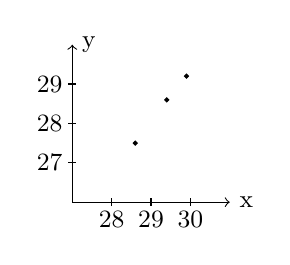
\begin{tikzpicture}[font=\small]
      \draw[<->](0,2) --(0,0)--(2,0);
      \draw (0.5, -0.05)--(0.5,0.05);
      \draw (1, -0.05)--(1,0.05);
      \draw (1.5, -0.05)--(1.5,0.05);
      \draw (-0.05, 0.5)--(0.05,0.5);
      \draw (-0.05, 1)--(0.05,1);
      \draw (-0.05, 1.5)--(0.05,1.5);
      \draw[fill] (0.8,0.75) circle [radius=0.025];
      \draw[fill] (1.2,1.3) circle [radius=0.025];
      \draw[fill] (1.45,1.6) circle [radius=0.025];
      \node[right] at (2,0){x};
      \node[right] at (0,2){y};
      \node[below] at (0.5,0){$28$};
      \node[below] at (1,0){$29$};
      \node[below] at (1.5,0){$30$};
      \node[left] at (0,0.5){$27$};
      \node[left] at (0,1){$28$};
      \node[left] at (0,1.5){$29$};
    \end{tikzpicture}
  \end{center}
\end{solution}

The following example demonstrates another system which exhibits some
interesting behavior. When we graph the solutions, it is possible for
the ordered pairs to spiral around the origin.

\begin{example}{Finding solutions to a dynamical system}{find-solutions-dynamical-system}
  Suppose a dynamical system is of the form
  \begin{equation*}
    \begin{mymatrix}{c}
      x(n+1) \\
      y(n+1)
    \end{mymatrix} =\begin{mymatrix}{rr}
      0.7 & 0.7 \\
      -0.7 & 0.7
    \end{mymatrix} \begin{mymatrix}{c}
      x(n) \\
      y(n)
    \end{mymatrix}.
  \end{equation*}
  Find solutions to the dynamical system for given initial conditions.
\end{example}

\begin{solution}
  Let
  \begin{equation*}
    A
    =
    \begin{mymatrix}{rr}
      0.7 & 0.7 \\
      -0.7 & 0.7
    \end{mymatrix}.
  \end{equation*}
  To find solutions, we must diagonalize $A$. You can verify that the
  eigenvalues of $A$ are complex and are given by
  $\eigenvar_1 = 0.7+0.7i$ and $\eigenvar_2 = 0.7-0.7i$. The eigenvector
  for $\eigenvar_1 = 0.7+0.7i$ is
  \begin{equation*}
    \begin{mymatrix}{r}
      1 \\
      i
    \end{mymatrix}
  \end{equation*}
  and that the eigenvector for $\eigenvar_2 = 0.7-0.7i$ is
  \begin{equation*}
    \begin{mymatrix}{r}
      1 \\
      -i
    \end{mymatrix}.
  \end{equation*}
  Thus the matrix $A$ can be written in the form
  \begin{equation*}
    \begin{mymatrix}{rr}
      1 & 1 \\
      i & -i
    \end{mymatrix} \begin{mymatrix}{cc}
      0.7+0.7i & 0 \\
      0 & 0.7-0.7i
    \end{mymatrix} \begin{mymatrix}{rr}
      \frac{1}{2} & -\frac{1}{2}i \\
      \frac{1}{2} & \frac{1}{2}i
    \end{mymatrix},
  \end{equation*}
  and so
  \begin{eqnarray*}
    V_n &=& PD^nP^{-1}V_0 \\
    \begin{mymatrix}{c}
      x(n) \\
      y(n)
    \end{mymatrix} &=&\begin{mymatrix}{rr}
      1 & 1 \\
      i & -i
    \end{mymatrix} \begin{mymatrix}{cc}
      (0.7+0.7i) ^{n} & 0 \\
      0 & (0.7-0.7i) ^{n}
    \end{mymatrix} \begin{mymatrix}{rr}
      \frac{1}{2} & -\frac{1}{2}i \\
      \frac{1}{2} & \frac{1}{2}i
    \end{mymatrix} \begin{mymatrix}{c}
      x_{0} \\
      y_{0}
    \end{mymatrix}.
  \end{eqnarray*}
  The explicit solution is given by
  \begin{equation*}
    \begin{mymatrix}{c}
      x_{0}(\frac{1}{2}(0.7-0.7i) ^{n}+\frac{1}{2}
      (0.7+0.7i) ^{n}) + \allowbreak y_{0}(\frac{1}{2}
      i(0.7-0.7i) ^{n}-\frac{1}{2}i (
      0.7+0.7i)  ^{n}) \\
      y_{0}(\frac{1}{2} (0.7-0.7i) ^{n}+\frac{1}{2}
      (0.7+0.7i) ^{n}) -  x_{0}(\frac{1}{2}
      i(0.7-0.7i) ^{n}-\frac{1}{2}i(
      0.7+0.7i) ^{n})
    \end{mymatrix}.
  \end{equation*}
  Suppose the initial condition is
  \begin{equation*}
    \begin{mymatrix}{c}
      x_{0} \\
      y_{0}
    \end{mymatrix} =\begin{mymatrix}{r}
      10 \\
      10
    \end{mymatrix}.
  \end{equation*}
  Then one obtains the following sequence of values which are graphed
  below by letting $n=1,2,\ldots,20$

  \begin{center}
    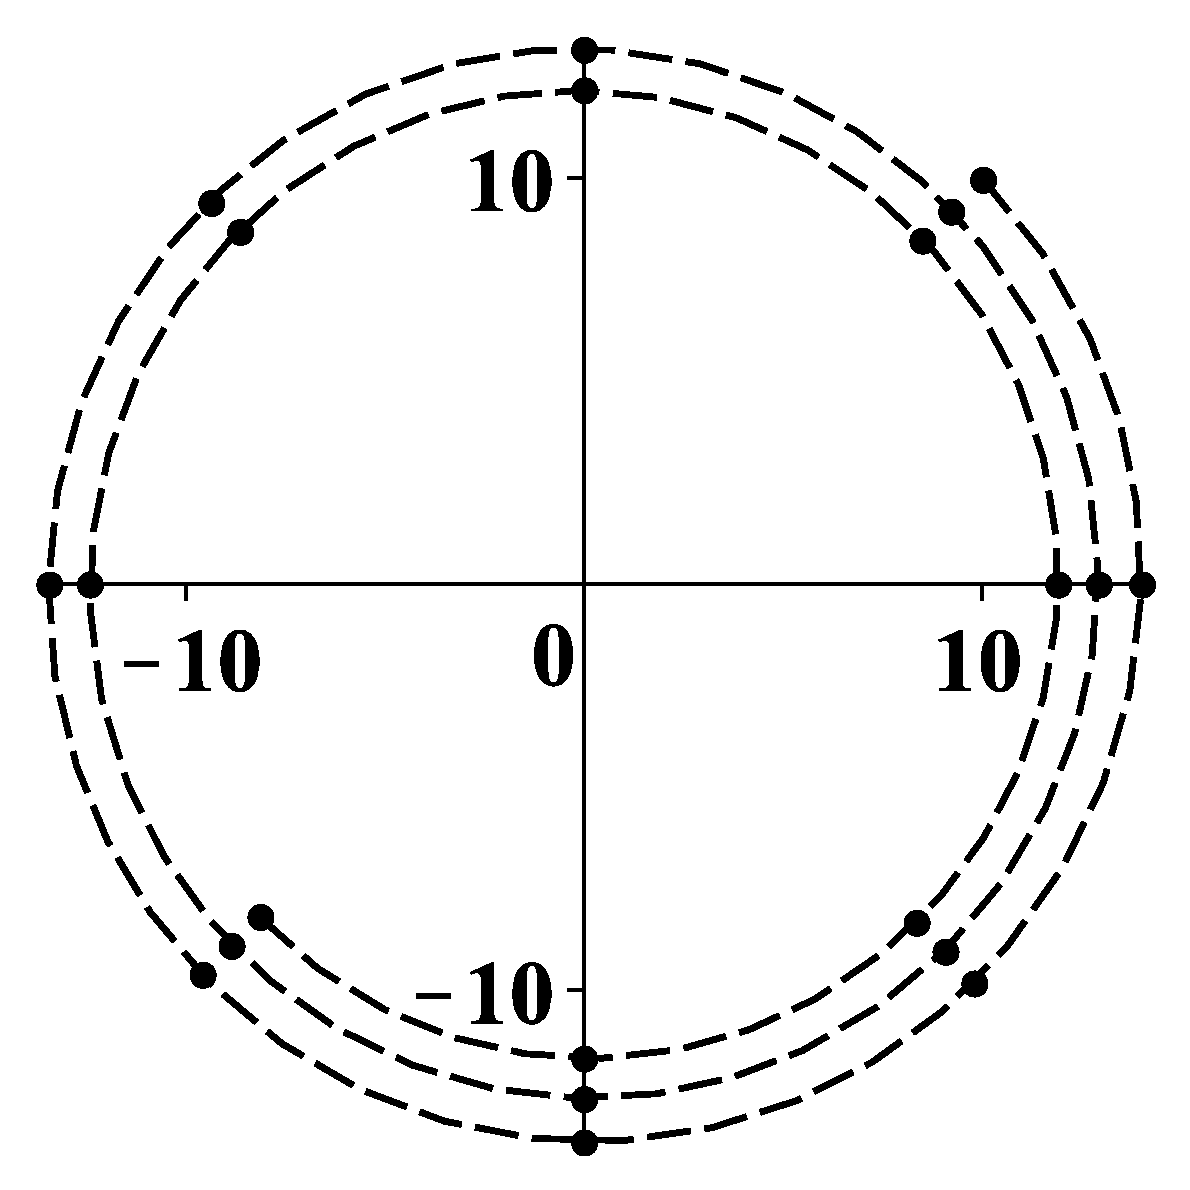
\includegraphics[bb=0 0 800 800,scale=.2]{figures/4dec.eps}
  \end{center}

  In this picture, the dots are the values and the dashed line is to
  help to picture what is happening.

  These points are getting gradually closer to the origin, but they
  are circling the origin in the clockwise direction as they do so. As
  $n$ increases, the vector $\begin{mymatrix}{c}
    x(n) \\
    y(n)
  \end{mymatrix}$ approaches $ \begin{mymatrix}{r}
    0 \\
    0
  \end{mymatrix}$.
\end{solution}

This type of behavior along with complex eigenvalues is typical of the
deviations from an equilibrium point in the Lotka Volterra system of
differential equations which is a famous model for predator-prey
interactions. These differential equations are given by
\begin{eqnarray*}
  x^{\prime } &=&x(a-by) \\
  y^{\prime } &=&-y(c-dx)
\end{eqnarray*}
where $a,b,c,d$ are positive constants. For example, you might have
$X$ be the population of moose and $Y$ the population of wolves on an
island.

Note that these equations make logical sense. The top says that the
rate at which the moose population increases would be $aX$ if there
were no predators $Y$.  However, this is modified by multiplying
instead by $(a-bY) $ because if there are predators, these will
militate against the population of moose.  The more predators there
are, the more pronounced is this effect. As to the predator equation,
you can see that the equations predict that if there are many prey
around, then the rate of growth of the predators would seem to be
high. However, this is modified by the term $-cY$ because if there are
many predators, there would be competition for the available food
supply and this would tend to decrease $Y^{\prime }$.

The behavior near an equilibrium point, which is a point where the
right side of the differential equations equals zero, is of great
interest. In this case, the equilibrium point is
\begin{equation*}
  x=\frac{c}{d}, y=\frac{a}{b}.
\end{equation*}
Then one defines new variables according to the formula
\begin{equation*}
  x+\frac{c}{d}=x,\ y=y+\frac{a}{b}.
\end{equation*}
In terms of these new variables, the differential equations become
\begin{eqnarray*}
  x^{\prime } &=&\paren{x+\frac{c}{d}} \paren{a-b\paren{y+\frac{a}{b}
                  }} \\
  y^{\prime } &=&-\paren{y+\frac{a}{b}} \paren{c-d\paren{x+\frac{c}{d}
                  }}.
\end{eqnarray*}
Multiplying out the right sides yields
\begin{eqnarray*}
  x^{\prime } &=&-bxy-b\frac{c}{d}y, \\
  y^{\prime } &=&dxy+\frac{a}{b}dx.
\end{eqnarray*}
The interest is for $x,y$ small and so these equations are essentially
equal to
\begin{equation*}
  x^{\prime }=-b\frac{c}{d}y,\ y^{\prime }=\frac{a}{b}dx.
\end{equation*}
Replace $x^{\prime }$ with the difference quotient
$\frac{x(t+h) -x(t) }{h}$ where $h$ is a small positive number and
$y^{\prime } $ with a similar difference quotient. For example one
could have $h$ correspond to one day or even one hour. Thus, for $h$
small enough, the following would seem to be a good approximation to
the differential equations.
\begin{eqnarray*}
  x(t+h) &=&x(t) -hb\frac{c}{d}y, \\
  y(t+h) &=&y(t) +h\frac{a}{b}dx.
\end{eqnarray*}
Let $1,2,3,\ldots$ denote the ends of discrete intervals of time
having length $h$ chosen above. Then the above equations take the form
\begin{equation*}
  \begin{mymatrix}{c}
    x(n+1) \\
    y(n+1)
  \end{mymatrix} =\begin{mymatrix}{cc}
    1 & -\frac{hbc}{d} \\
    \frac{had}{b} & 1
  \end{mymatrix} \begin{mymatrix}{c}
    x(n) \\
    y(n).
  \end{mymatrix}
\end{equation*}
Note that the eigenvalues of this matrix are always complex.

We are not interested in time intervals of length $h$ for $h$ very
small.  Instead, we are interested in much longer lengths of
time. Thus, replacing the time interval with $mh$,
\begin{equation*}
  \begin{mymatrix}{c}
    x(n+m) \\
    y(n+m)
  \end{mymatrix} =\begin{mymatrix}{cc}
    1 & -\frac{hbc}{d} \\
    \frac{had}{b} & 1
  \end{mymatrix} ^{m}\begin{mymatrix}{c}
    x(n) \\
    y(n)
  \end{mymatrix}.
\end{equation*}
For example, if $m=2$, you would have
\begin{equation*}
  \begin{mymatrix}{c}
    x(n+2) \\
    y(n+2)
  \end{mymatrix} =\begin{mymatrix}{cc}
    1-ach^{2} & -2b\frac{c}{d}h \\
    2\frac{a}{b}dh & 1-ach^{2}
  \end{mymatrix} \begin{mymatrix}{c}
    x(n) \\
    y(n)
  \end{mymatrix}.
\end{equation*}
Note that most of the time, the eigenvalues of the new matrix will be
complex.

You can also notice that the upper right corner will be negative by
considering higher powers of the matrix. Thus letting $1,2,3,\ldots$
denote the ends of discrete intervals of time, the desired discrete
dynamical system is of the form
\begin{equation*}
  \begin{mymatrix}{c}
    x(n+1) \\
    y(n+1)
  \end{mymatrix} =\begin{mymatrix}{rr}
    a & -b \\
    c & d
  \end{mymatrix} \begin{mymatrix}{c}
    x(n) \\
    y(n)
  \end{mymatrix},
\end{equation*}
where $a,b,c,d$ are positive constants and the matrix will likely have
complex eigenvalues because it is a power of a matrix which has
complex eigenvalues.

You can see from the above discussion that if the eigenvalues of the
matrix used to define the dynamical system are less than 1 in absolute
value, then the origin is stable in the sense that as
$n\rightarrow \infty$, the solution converges to the origin. If either
eigenvalue is larger than 1 in absolute value, then the solutions to
the dynamical system will usually be unbounded, unless the initial
condition is chosen very carefully. The next example exhibits the case
where one eigenvalue is larger than 1 and the other is smaller than 1.

The following example demonstrates a familiar concept as a dynamical system.
